\documentclass[11pt]{article}

\usepackage[T1]{fontenc}
\usepackage{lmodern}
\usepackage[margin=2.4cm]{geometry}
\usepackage{amsmath,amssymb}
\usepackage{graphicx}
\usepackage{booktabs}
\usepackage{tabularx}
\usepackage{xurl}
\usepackage[hidelinks]{hyperref}
\usepackage[section]{placeins}

\renewcommand{\thesection}{S\arabic{section}}
\renewcommand{\thetable}{S\arabic{table}}
\renewcommand{\thefigure}{S\arabic{figure}}
\renewcommand{\theequation}{S\arabic{equation}}
\newcommand{\tablesetup}{\small\setlength{\tabcolsep}{4pt}}

\title{Supplementary material\\[4pt]
\large Training parts versus matching parts in pose-based gait recognition}
\author{Minas Aslanyan \and Levon Aslanyan}
\date{}

\begin{document}
\maketitle

\noindent Section, table and figure numbers without the prefix ``S'' refer to the
main article. All values are Rank-1 in percent or Rank-1 differences in
percentage points unless stated otherwise. Every table except Tables~S1--S3 is
generated by \texttt{make\_tables.py} from \texttt{evidence\_pr.json}, which
\texttt{build\_pr\_evidence.py} assembles from the saved run artifacts.

\section{Three-seed factorial}
\label{sec:s-factorial}

The factorial trained six objectives with seeds 11, 22 and 33 under source
revision \texttt{ad96b902\ldots}; the five-seed cohort in the main text used
revision \texttt{11b575d0\ldots}. Both used the same recipe, identities and
evaluation masks. Tables~S1 and S2 report the factorial with the global and the
learned projected-parts descriptors; its intervals use a crossed bootstrap with
100,000 draws. In this cohort part SupCon reduced the corrupted-probe aggregate
by 6.12 points, $[-10.29,-2.00]$. The five-seed cohort estimates the same
contrast at $-1.27$, $[-5.24,2.74]$ (main Table~3), so the main text does not
retain a harmful effect of part SupCon.

Table~S3 lists training diagnostics. The part-triplet objective closely
preserved clean global accuracy but its final normalized part variance was
about $1.7\times10^{-6}$; at the selected epochs (60, 60 and 40) the variance
averaged $2.03\times10^{-6}$ across seeds and parts, and a nonzero finite
part--triplet gradient cosine was available in only 9 of 96 scheduled
measurements (the remainder had a zero-norm gradient for at least one compared
loss). These observations indicate near-collapse of the local embeddings under
this objective and recipe. Part SupCon avoided collapse (variance
$3.34\times10^{-3}$), but in the combined model its gradient agreed less with
the global triplet objective than the global SupCon gradient did (mean cosines
0.203 and 0.446). The cosines are positive, so the data do not show direct
gradient opposition. Cosines are measured at the shared paired-view feature
tensor, and variance diagnostics describe training batches rather than test
embeddings.

% Copied verbatim from the verified IJCV manuscript (Paper/IJCV/main.tex); only float type, labels and caption prefixes changed.
\begin{table}[!htbp]
\centering
\caption{Three-seed factorial (earlier source revision). CASIA-B validation Rank-1 (\%). Clean is mean $\pm$ seed standard
deviation. ``All $>0$'' averages four corruption families at severities 0.1,
0.3, 0.5, and 0.7. Occluded gallery averages the same positive-severity grid.
Single-view averages NM, BG, and CL. Every cell uses three training seeds.}
\label{tab:s-factorial}
\small
\setlength{\tabcolsep}{4pt}
\begin{tabularx}{\textwidth}{@{}>{\raggedright\arraybackslash}Xccccc@{}}
\toprule
\multicolumn{6}{@{}l}{\emph{Global descriptor}} \\
Training objective & Clean & \shortstack{Clean gallery\\all $>0$} &
\shortstack{Clean gallery\\$\rho=0.5$} & \shortstack{Occluded gallery\\all $>0$} &
Single-view \\
\midrule
Metric baseline & 81.52 $\pm$ 2.43 & 63.90 & 64.25 & 67.93 & 67.36 \\
Global SupCon & 79.63 $\pm$ 3.23 & 63.23 & 64.15 & 67.42 & 66.18 \\
Part SupCon & 78.79 $\pm$ 1.14 & 57.78 & 55.57 & 64.26 & 65.33 \\
Part triplet & 81.27 $\pm$ 3.41 & 60.65 & 59.10 & 66.71 & 67.82 \\
Global + part SupCon & 80.05 $\pm$ 1.34 & 60.70 & 59.06 & 65.56 & 65.75 \\
Global + part SupCon (ungated) & 80.89 $\pm$ 1.59 & 61.72 & 60.59 & 66.99 & 66.29 \\
\bottomrule
\end{tabularx}
\vspace{0.5em}

\begin{tabularx}{\textwidth}{@{}>{\raggedright\arraybackslash}Xccccc@{}}
\toprule
\multicolumn{6}{@{}l}{\emph{Projected-parts descriptor}} \\
Training objective & Clean & \shortstack{Clean gallery\\all $>0$} &
\shortstack{Clean gallery\\$\rho=0.5$} & \shortstack{Occluded gallery\\all $>0$} &
Single-view \\
\midrule
Metric baseline & 83.04 $\pm$ 1.31 & 66.31 & 67.97 & 70.57 & 69.34 \\
Global SupCon & 82.79 $\pm$ 3.36 & 66.21 & 67.85 & 70.38 & 68.66 \\
Part SupCon & 75.42 $\pm$ 2.25 & 54.66 & 52.65 & 61.62 & 61.81 \\
Part triplet & 81.31 $\pm$ 3.42 & 60.66 & 59.11 & 66.73 & 67.82 \\
Global + part SupCon & 77.86 $\pm$ 4.45 & 57.48 & 54.84 & 63.18 & 63.40 \\
Global + part SupCon (ungated) & 78.20 $\pm$ 0.07 & 59.35 & 58.11 & 64.85 & 65.60 \\
\bottomrule
\end{tabularx}
\end{table}

\begin{table}[!htbp]
\centering
\caption{Three-seed factorial. Paired Rank-1 difference from the metric baseline in percentage points
(crossed 95\% bootstrap interval over seed and validation identity).
Negative values favor the baseline.}
\label{tab:s-factorial-paired}
\small
\setlength{\tabcolsep}{4pt}
\begin{tabularx}{\textwidth}{@{}>{\raggedright\arraybackslash}Xlcc@{}}
\toprule
Training objective & Descriptor & Clean & \shortstack{Clean gallery,\\all $>0$} \\
\midrule
Global SupCon & Global & -1.89 [-5.30, +1.05] & -0.67 [-4.86, +3.79] \\
Part SupCon & Global & -2.74 [-6.69, +1.18] & -6.12 [-10.29, -2.00] \\
Part triplet & Global & -0.25 [-5.22, +4.17] & -3.26 [-7.59, +1.06] \\
Global + part SupCon & Global & -1.47 [-5.85, +3.03] & -3.21 [-8.97, +2.89] \\
Global + part (ungated) & Global & -0.63 [-5.35, +5.30] & -2.19 [-5.35, +1.11] \\
Global SupCon & Projected parts & -0.25 [-3.79, +2.99] & -0.10 [-3.27, +3.08] \\
Part SupCon & Projected parts & -7.62 [-11.91, -3.03] & -11.65 [-16.02, -7.32] \\
Part triplet & Projected parts & -1.73 [-6.82, +2.90] & -5.65 [-9.85, -1.16] \\
Global + part SupCon & Projected parts & -5.18 [-10.61, +0.13] & -8.83 [-14.35, -2.29] \\
Global + part (ungated) & Projected parts & -4.84 [-8.75, -1.05] & -6.96 [-11.01, -3.08] \\
\bottomrule
\end{tabularx}
\vspace{0.5em}

\begin{tabularx}{\textwidth}{@{}>{\raggedright\arraybackslash}Xlcc@{}}
\toprule
Training objective & Descriptor & \shortstack{Clean gallery,\\$\rho=0.5$} &
\shortstack{Occluded gallery,\\all $>0$} \\
\midrule
Global SupCon & Global & -0.10 [-6.13, +6.76] & -0.51 [-2.90, +1.76] \\
Part SupCon & Global & -8.68 [-15.55, -2.38] & -3.67 [-6.00, -1.27] \\
Part triplet & Global & -5.15 [-11.42, +1.28] & -1.22 [-4.29, +1.50] \\
Global + part SupCon & Global & -5.19 [-13.69, +4.17] & -2.37 [-6.16, +1.24] \\
Global + part (ungated) & Global & -3.65 [-8.91, +0.68] & -0.94 [-3.00, +1.05] \\
Global SupCon & Projected parts & -0.12 [-4.37, +4.10] & -0.20 [-2.13, +1.76] \\
Part SupCon & Projected parts & -15.32 [-22.19, -8.96] & -8.96 [-11.51, -6.03] \\
Part triplet & Projected parts & -8.86 [-15.80, -1.57] & -3.85 [-6.48, -1.32] \\
Global + part SupCon & Projected parts & -13.13 [-20.45, -4.51] & -7.39 [-11.19, -2.97] \\
Global + part (ungated) & Projected parts & -9.85 [-16.07, -4.53] & -5.73 [-8.08, -3.59] \\
\bottomrule
\end{tabularx}
\end{table}

\begin{table}[!htbp]
\centering
\caption{Three-seed factorial. Training diagnostics averaged over three seeds. Part variance is the
mean coordinate-wise variance over the final 20 epochs. Cosines are measured
every five epochs; parentheses give nonzero finite cosine measurements out of
96 scheduled.}
\label{tab:s-diagnostics}
\small
\setlength{\tabcolsep}{4pt}
\begin{tabular}{@{}lrrr@{}}
\toprule
Objective & Variance ($\times10^{-3}$) & Part--global & Part--triplet \\
\midrule
Metric baseline & 1.269 & -- & -- \\
Global SupCon & 1.300 & -- & -- \\
Part SupCon & 3.338 & -- & 0.212 (95) \\
Part triplet & 0.002 & -- & 0.012 (9) \\
Global + part SupCon & 3.349 & 0.265 (96) & 0.203 (96) \\
Global + part SupCon (ungated) & 3.242 & 0.241 (96) & 0.195 (96) \\
\bottomrule
\end{tabular}
\end{table}


\section{Corruption calibration and evaluation matrix}
\label{sec:s-corruption}

Nominal severity $\rho$ is the requested missing fraction. Whole-part masks
remove complete anatomical regions and overshoot small requests, while
temporal smoothing lowers the marginal dynamic-joint rate at small $\rho$ and
raises it at large $\rho$. Table~S4 gives the removed fraction of real
joint-frames, regenerated exactly as the evaluator drew each mask from its
recorded seed, family order, realization and probe index. Figure~S1 records
where each family is used, and Figure~S2 illustrates the four families.

\begin{table}[!htbp]
\centering
\caption{Mean removed fraction of observed joint-frames (\%) at each nominal
severity, CASIA-B development probes / Gait3D development probes.}
\label{tab:s-missingness}
{\tablesetup
% Generated by make_tables.py from evidence_pr.json; do not edit by hand.
\begin{tabular}{@{}lcccc@{}}
\toprule
Family & $\rho=0.1$ & $\rho=0.3$ & $\rho=0.5$ & $\rho=0.7$ \\
\midrule
Random joint-frame & 10.0 / 10.0 & 30.0 / 30.0 & 50.0 / 50.0 & 70.0 / 70.0 \\
Dynamic joint & 3.2 / 3.2 & 22.3 / 22.4 & 50.6 / 50.7 & 78.7 / 78.8 \\
Whole part & 18.8 / 18.9 & 35.3 / 35.3 & 49.4 / 49.3 & 70.6 / 70.6 \\
Temporal interruption & 10.0 / 10.0 & 30.0 / 30.0 & 50.0 / 50.0 & 70.0 / 70.0 \\
\bottomrule
\end{tabular}
}
\end{table}

\begin{figure}[!htbp]
\centering
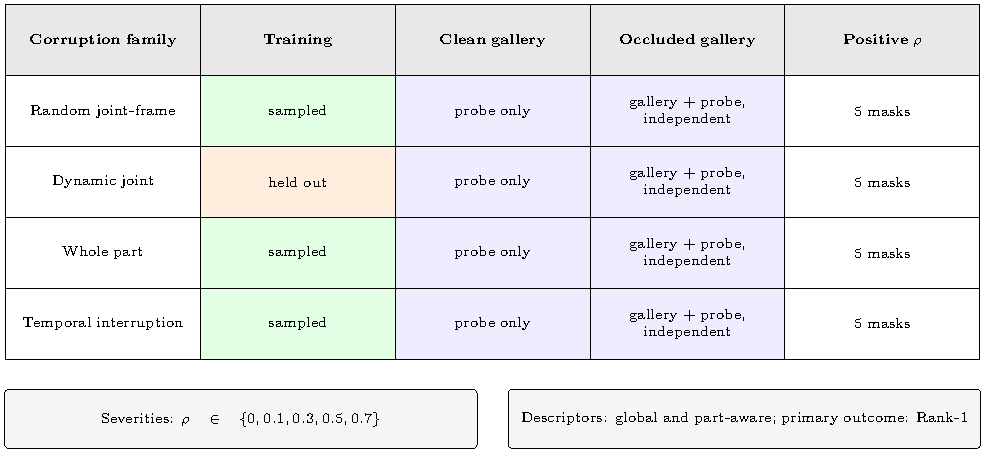
\includegraphics[width=\textwidth]{figS1.pdf}
\caption{Evaluation matrix. Dynamic-joint corruption is held out from
training. Positive-severity results average five deterministic corruption
realizations, and gallery and probe corruptions are independently seeded in the
occluded-gallery protocol.}
\label{fig:s-matrix}
\end{figure}

\begin{figure}[!htbp]
\centering
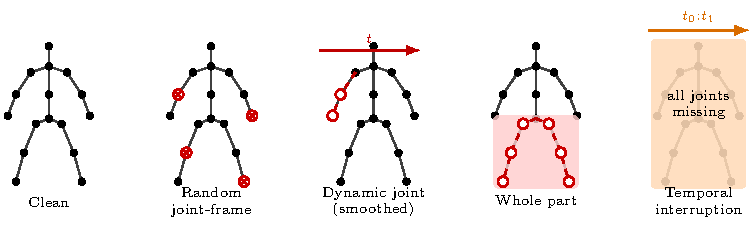
\includegraphics[width=\textwidth]{figS2.pdf}
\caption{Corruption families. Red marks unavailable joints or regions; orange
marks a contiguous interval without pose. Random joint-frame masks vary
independently, whereas dynamic-joint masks are temporally smoothed.}
\label{fig:s-families}
\end{figure}

\section{Fusion-weight sensitivity}
\label{sec:s-weights}

The local-score weight $\lambda$ was declared as 0.5 before any comparison.
Table~S5 shows the reliability-weighted raw-part matcher on the frozen
metric-baseline checkpoints at all five evaluated weights; $\lambda=0$ is the
global descriptor. The best CASIA-B weight (0.75) would have removed the
Gait3D gain, and part-only matching ($\lambda=1$) is markedly worse than the
global descriptor on Gait3D.

\begin{table}[!htbp]
\centering
\caption{Raw reliability-weighted part matching on frozen metric-baseline
checkpoints at different local-score weights, Rank-1 (\%).}
\label{tab:s-weights}
{\tablesetup
% Generated by make_tables.py from evidence_pr.json; do not edit by hand.
\begin{tabular}{@{}lcccc@{}}
\toprule
 & \multicolumn{2}{c}{CASIA-B, five seeds} & \multicolumn{2}{c}{Gait3D, three seeds} \\
\cmidrule(lr){2-3}\cmidrule(l){4-5}
Local-score weight $\lambda$ & Clean & Corr.\ probe & Clean & Corr.\ probe \\
\midrule
0.0 & $79.60$ & $60.93$ & $35.89$ & $23.96$ \\
0.25 & $81.19$ & $62.97$ & $36.67$ & $25.26$ \\
0.5 (declared) & $82.40$ & $64.66$ & $36.89$ & $25.81$ \\
0.75 & $83.43$ & $65.71$ & $33.67$ & $23.87$ \\
1.0 & $84.37$ & $65.20$ & $21.33$ & $15.07$ \\
\bottomrule
\end{tabular}
}
\end{table}

\section{Raw matching for every trained objective}
\label{sec:s-raw}

Table~S6 lists the values plotted in main Figure~3: raw reliability-weighted
part matching minus global matching from the same checkpoints, with crossed
seed-by-identity bootstrap intervals (20,000 draws).

\begin{table}[!htbp]
\centering
\caption{Raw reliability-weighted part matching minus global matching (Rank-1
points, crossed 95\% intervals), from each training run's own evaluation. The
checkpoint-control analysis in main Table~4 re-encodes the metric-baseline
checkpoints and differs from these values by at most 0.05 points.}
\label{tab:s-raw}
{\tablesetup\footnotesize
% Generated by make_tables.py from evidence_pr.json; do not edit by hand.
\begin{tabular}{@{}llccc@{}}
\toprule
Cohort & Training objective & Clean & Corr.\ probe & Corr.\ gallery \\
\midrule
CASIA-B, 5 seeds & CE, no masking & ${+}2.53$ [0.61, 4.75] & ${+}2.32$ [1.47, 3.24] & ${+}3.50$ [2.60, 4.34] \\
CASIA-B, 5 seeds & Masked CE & ${+}2.85$ [1.26, 4.39] & ${+}3.48$ [2.23, 4.63] & ${+}3.54$ [2.72, 4.33] \\
CASIA-B, 5 seeds & Matched CE & ${+}1.44$ [$-$0.18, 3.23] & ${+}3.21$ [1.74, 4.69] & ${+}2.61$ [1.71, 3.60] \\
CASIA-B, 5 seeds & Metric baseline & ${+}2.75$ [0.38, 4.75] & ${+}3.73$ [1.67, 5.68] & ${+}3.66$ [2.12, 5.06] \\
CASIA-B, 5 seeds & Global SupCon & ${+}2.68$ [0.88, 4.70] & ${+}4.28$ [2.79, 5.92] & ${+}3.83$ [2.87, 4.81] \\
CASIA-B, 5 seeds & Part SupCon & ${+}1.89$ [0.18, 3.69] & ${+}2.87$ [1.32, 4.31] & ${+}2.70$ [1.96, 3.41] \\
CASIA-B, 5 seeds & Global + part SupCon & ${+}1.94$ [0.48, 3.54] & ${+}2.95$ [1.96, 4.10] & ${+}2.73$ [2.06, 3.49] \\
\midrule
Gait3D dev., 3 seeds & CE, no masking & $-1.00$ [$-$3.78, 1.67] & ${+}0.90$ [0.49, 1.33] & ${+}0.86$ [0.46, 1.26] \\
Gait3D dev., 3 seeds & Matched CE & ${+}0.33$ [$-$2.33, 2.89] & ${+}2.25$ [1.10, 3.43] & ${+}1.64$ [0.70, 2.62] \\
Gait3D dev., 3 seeds & Metric baseline & ${+}1.00$ [$-$2.56, 4.67] & ${+}1.85$ [0.76, 2.98] & ${+}1.57$ [0.71, 2.50] \\
Gait3D dev., 3 seeds & Global + part SupCon & ${+}1.44$ [$-$1.00, 4.00] & ${+}2.02$ [1.03, 3.01] & ${+}1.72$ [0.95, 2.50] \\
\midrule
Gait3D test, 5 seeds & CE, no masking & ${+}1.46$ [0.44, 2.47] & ${+}0.60$ [0.44, 0.76] & ${+}0.71$ [0.52, 0.90] \\
Gait3D test, 5 seeds & Metric baseline & ${+}1.99$ [0.61, 3.38] & ${+}1.59$ [1.07, 2.12] & ${+}1.19$ [0.76, 1.63] \\
\bottomrule
\end{tabular}
}
\end{table}

\section{Additional development results}
\label{sec:s-dev}

Table~S7 breaks the five-seed CASIA-B single-view average of main Table~2 into
its normal, bag and clothing conditions. Table~S8 gives the Gait3D development
results by objective (300 held-out training identities, one probe each, three
seeds).

\begin{table}[!htbp]
\centering
\caption{CASIA-B development, single-view-gallery protocol excluding identical
views, five seeds (mean $\pm$ seed standard deviation).}
\label{tab:s-single-view}
{\tablesetup\footnotesize
% Generated by make_tables.py from evidence_pr.json; do not edit by hand.
\begin{tabular}{@{}lcccccc@{}}
\toprule
 & \multicolumn{3}{c}{Global descriptor} & \multicolumn{3}{c}{Raw parts, reliability-weighted} \\
\cmidrule(lr){2-4}\cmidrule(l){5-7}
Training objective & NM & BG & CL & NM & BG & CL \\
\midrule
CE, no masking & $76.77\pm1.40$ & $58.30\pm2.40$ & $53.29\pm3.69$ & $80.80\pm1.67$ & $61.69\pm3.43$ & $56.96\pm4.06$ \\
Masked CE & $65.27\pm3.37$ & $46.11\pm2.51$ & $39.98\pm3.75$ & $69.30\pm2.84$ & $48.61\pm2.34$ & $41.90\pm3.29$ \\
Matched CE & $79.99\pm3.59$ & $62.01\pm3.23$ & $54.48\pm1.40$ & $83.47\pm2.96$ & $63.81\pm2.71$ & $56.77\pm2.73$ \\
Metric baseline & $79.52\pm1.38$ & $59.25\pm3.21$ & $57.56\pm2.80$ & $83.20\pm1.20$ & $62.05\pm1.98$ & $59.83\pm1.83$ \\
Global SupCon & $79.42\pm2.06$ & $61.23\pm1.20$ & $59.25\pm3.07$ & $83.52\pm1.37$ & $63.97\pm1.33$ & $61.17\pm3.53$ \\
Part SupCon & $77.97\pm1.07$ & $61.11\pm2.83$ & $53.02\pm2.25$ & $81.33\pm1.23$ & $62.89\pm1.82$ & $54.52\pm3.00$ \\
Global + part SupCon & $78.18\pm2.50$ & $59.68\pm2.74$ & $58.48\pm1.54$ & $81.11\pm1.72$ & $62.34\pm3.18$ & $60.49\pm1.48$ \\
\bottomrule
\end{tabular}
}
\end{table}

\begin{table}[!htbp]
\centering
\caption{Gait3D development Rank-1 (\%), three seeds, 300 probes (mean $\pm$
seed standard deviation where shown).}
\label{tab:s-gait3d-dev}
{\tablesetup
% Generated by make_tables.py from evidence_pr.json; do not edit by hand.
\begin{tabular}{@{}lccccc@{}}
\toprule
 & \multicolumn{3}{c}{Global descriptor} & \multicolumn{2}{c}{Raw parts, reliability-weighted} \\
\cmidrule(lr){2-4}\cmidrule(l){5-6}
Training objective & Clean & Corr.\ probe & Corr.\ gallery & Clean & Corr.\ probe \\
\midrule
CE, no masking & $28.44\pm2.55$ & $8.26\pm0.50$ & $9.58$ & $27.44$ & $9.15$ \\
Matched CE & $31.56\pm1.92$ & $21.50\pm0.92$ & $19.24$ & $31.89$ & $23.74$ \\
Metric baseline & $35.89\pm2.55$ & $23.96\pm1.26$ & $21.39$ & $36.89$ & $25.81$ \\
Global + part SupCon & $34.44\pm1.71$ & $24.03\pm0.64$ & $21.84$ & $35.89$ & $26.05$ \\
\bottomrule
\end{tabular}
}
\end{table}

\section{GPGait transfer: variants and fusion weights}
\label{sec:s-gpgait}

Features were extracted with \texttt{scripts/fpg\_part\_matching.py}, which
runs each trained GPGait checkpoint through FastPoseGait's own test loader,
transforms and network code and records the 19 inference embeddings and the
per-joint features of each branch's global backbone after temporal pooling.
GPGait creates every graph layer's learnable adjacency from one shared tensor;
the script copies each parameter before loading the checkpoint, as
FastPoseGait's transfer to the GPU does, and refuses to run if parameters still
share storage. With all 19 embeddings it reproduces the logged CASIA-B results
(93.78, 79.89 and 69.12 against 93.77, 79.86 and 69.11) and Gait3D Rank-1
(23.13). Table~S9 adds the exploratory variant that passes mean-plus-max region
pools through each branch's trained whole-body projection and BNNeck layer
(maximum reconstruction error of GPGait's own whole-body embeddings
$7\times10^{-4}$) and fusion weights 0.25 and 0.75. No variant or weight lets
raw parts improve on the full descriptor; at $\lambda=0.25$ they change the
whole-body descriptor by less than 0.5 points.

\begin{table}[!htbp]
\centering
\caption{GPGait with raw parts: declared and exploratory variants and other
fusion weights (Rank-1 and mAP, \%). Without raw parts, the full descriptor
reaches 80.93 (CASIA-B average) and 23.13 / 16.79 (Gait3D Rank-1 / mAP), and the
whole-body descriptor 71.85 and 17.95 / 12.59.}
\label{tab:s-gpgait}
{\tablesetup\footnotesize
% Generated by make_tables.py from evidence_pr.json; do not edit by hand.
\begin{tabular}{@{}lccc@{}}
\toprule
Descriptor & CASIA-B average & Gait3D Rank-1 & Gait3D mAP \\
\midrule
\multicolumn{4}{@{}l}{\emph{Declared: mean pool, no projection}} \\
Raw parts only & $16.20$ & $9.40$ & $6.20$ \\
Whole-body + raw & $70.92$ & $17.11$ & $11.86$ \\
Full + raw & $78.53$ & $19.96$ & $14.24$ \\
Whole-body + raw, $\lambda=0.25$ & $72.00$ & $17.53$ & $12.55$ \\
Full + raw, $\lambda=0.25$ & $80.70$ & $22.28$ & $15.64$ \\
Whole-body + raw, $\lambda=0.75$ & $63.16$ & $16.16$ & $10.62$ \\
Full + raw, $\lambda=0.75$ & $65.75$ & $16.47$ & $11.43$ \\
\midrule
\multicolumn{4}{@{}l}{\emph{Exploratory: mean+max pool through the whole-body head}} \\
Raw parts only & $36.07$ & $12.46$ & $8.92$ \\
Whole-body + raw & $71.29$ & $16.58$ & $11.83$ \\
Full + raw & $77.61$ & $18.90$ & $13.37$ \\
Whole-body + raw, $\lambda=0.25$ & $72.21$ & $17.63$ & $12.38$ \\
Full + raw, $\lambda=0.25$ & $80.59$ & $21.65$ & $15.34$ \\
Whole-body + raw, $\lambda=0.75$ & $62.91$ & $14.57$ & $10.53$ \\
Full + raw, $\lambda=0.75$ & $64.55$ & $15.84$ & $11.07$ \\
\bottomrule
\end{tabular}
}
\end{table}

\section{Detector-confidence stratification on Gait3D}
\label{sec:s-confidence}

Gait3D has no occlusion annotation. Each development probe is described by
proxies computed only from its released HRNet confidences over the real frames
the evaluator embeds: the fraction of joint-frames with confidence below 0.5
(primary), the fraction below 0.3, one minus the mean confidence, and one minus
the lowest mean part confidence. The primary proxy, threshold and endpoints were
fixed from the confidence and height distributions before outcomes were
examined; at threshold 0.3 a fifth of probes have no qualifying joint-frame.
The primary endpoint is the height-matched interaction: within each
skeleton-height tertile, probes are split into tertiles of the primary proxy,
the raw-minus-global Rank-1 gain among the most low-confidence probes minus the
gain among the least is computed, and the three height strata are averaged with
equal weight. The secondary endpoint repeats the contrast over global tertiles.
Intervals resample training seeds and probe identities as crossed clusters
(20,000 draws). The tertile edges of the primary proxy are 1.65\% and 4.28\% of
joint-frames (range 0.09--19.7\%), and its Spearman correlations with
sequence length and skeleton height are $-0.05$ and $-0.29$. The primary
endpoint is $-0.68$ points, $[-7.69,6.22]$, and the secondary $+1.00$ points,
$[-6.54,8.45]$. Low confidence also follows resolution and blur, bins use probe
evidence only, and gallery tracks may themselves be occluded; the analysis
therefore cannot establish whether the matching gain addresses real
occlusion.

\section{Test-set details}
\label{sec:s-test}

Main Table~5 reports means. Tables~S10 and~S11 add seed standard deviations,
the uniform-weight raw descriptor, Rank-5, Rank-10, mINP and parameter counts,
and Table~S12 gives the paired intervals for the GPGait descriptor variants.

\begin{table}[!htbp]
\centering
\caption{CASIA-B official test (identities 075--124), standard single-view
protocol excluding identical views, Rank-1 (\%). Our rows give mean $\pm$
standard deviation over five seeds of the metric baseline; reproduced
baselines were trained once with official FastPoseGait configurations, and
reported values are those of the FastPoseGait model zoo. Parameters include
each model's identity classifier.}
\label{tab:s-casia-test}
{\tablesetup\footnotesize
% Generated by make_tables.py from evidence_pr.json; do not edit by hand.
\begin{tabular}{@{}lccccc@{}}
\toprule
System & NM & BG & CL & Average & \begin{tabular}[b]{@{}c@{}}Params.\\(M)\end{tabular} \\
\midrule
Ours, global & $67.64\pm2.83$ & $49.50\pm1.92$ & $27.91\pm0.94$ & $48.35\pm1.85$ & $1.69$ \\
Ours, raw (uniform) & $74.02\pm3.04$ & $55.56\pm2.04$ & $32.54\pm1.88$ & $54.04\pm2.21$ & $1.69$ \\
Ours, raw (reliability) & $74.14\pm3.04$ & $55.47\pm2.01$ & $32.52\pm1.81$ & $54.04\pm2.18$ & $1.69$ \\
\midrule
GaitGraph2 (reproduced) & $76.66$ & $67.23$ & $60.63$ & $68.17$ & $0.35$ \\
GaitGraph2 (reported) & $80.29$ & $71.40$ & $63.80$ & $71.83$ & -- \\
GPGait (reproduced) & $93.77$ & $79.86$ & $69.11$ & $80.91$ & $3.65$ \\
GPGait (reported) & $93.60$ & $80.15$ & $69.29$ & $81.01$ & -- \\
\bottomrule
\end{tabular}
}
\end{table}

\begin{table}[!htbp]
\centering
\caption{Gait3D test, available-pose subset (947 probes, 5,122 gallery
sequences), evaluated once. Our rows give means over five seeds ($\pm$ seed
standard deviation for Rank-1 and mAP). ``Metric'' is the metric baseline and
``raw'' the raw-part descriptor. Parameters include the 2,892-way identity
classifier where present.}
\label{tab:s-gait3d-test}
{\tablesetup\footnotesize
% Generated by make_tables.py from evidence_pr.json; do not edit by hand.
\begin{tabular}{@{}lcccccc@{}}
\toprule
System & Rank-1 & Rank-5 & Rank-10 & mAP & mINP & \begin{tabular}[b]{@{}c@{}}Params.\\(M)\end{tabular} \\
\midrule
CE, global & $15.48\pm1.38$ & $30.41$ & $38.46$ & $12.07\pm0.40$ & $7.16$ & $2.41$ \\
CE, raw (reliability) & $16.94\pm1.26$ & $31.89$ & $39.64$ & $12.87\pm0.51$ & $7.91$ & $2.41$ \\
Metric, global & $21.88\pm1.18$ & $38.94$ & $46.99$ & $16.89\pm0.43$ & $10.17$ & $2.41$ \\
Metric, raw (uniform) & $23.86\pm0.64$ & $39.94$ & $47.79$ & $17.82\pm0.24$ & $10.90$ & $2.41$ \\
Metric, raw (reliability) & $23.86\pm0.68$ & $40.02$ & $47.69$ & $17.79\pm0.24$ & $10.86$ & $2.41$ \\
\midrule
GaitGraph2 (reproduced) & $8.87$ & $24.50$ & $31.47$ & $8.38$ & $4.77$ & $0.35$ \\
GPGait (reproduced) & $23.13$ & $36.43$ & $44.14$ & $16.78$ & $10.51$ & $18.11$ \\
\bottomrule
\end{tabular}
}
\end{table}

\begin{table}[!htbp]
\centering
\caption{Raw part matching applied to GPGait, with paired differences. ``Full''
is the published descriptor and W its three whole-body embeddings; raw parts are
fused at $\lambda=0.5$ on GPGait's native distance. Intervals resample test
identities.}
\label{tab:s-gpgait-paired}
{\tablesetup\footnotesize
% Generated by make_tables.py from evidence_pr.json; do not edit by hand.
\begin{tabular}{@{}lcccccc@{}}
\toprule
 & \multicolumn{4}{c}{CASIA-B official test} & \multicolumn{2}{c}{Gait3D test} \\
\cmidrule(lr){2-5}\cmidrule(l){6-7}
GPGait descriptor & NM & BG & CL & Average & Rank-1 & mAP \\
\midrule
Full (19 embeddings) & $93.78$ & $79.89$ & $69.12$ & $80.93$ & $23.13$ & $16.79$ \\
Whole-body only (W) & $87.86$ & $68.21$ & $59.49$ & $71.85$ & $17.95$ & $12.59$ \\
Raw parts only & $22.12$ & $14.85$ & $11.62$ & $16.20$ & $9.40$ & $6.20$ \\
W + raw parts & $86.53$ & $67.15$ & $59.07$ & $70.92$ & $17.11$ & $11.86$ \\
Full + raw parts & $91.55$ & $77.01$ & $67.05$ & $78.53$ & $19.96$ & $14.24$ \\
\midrule
\multicolumn{7}{@{}l}{\emph{Paired differences (points), 95\% interval over test identities}} \\
W $-$ full & \multicolumn{4}{c}{$-9.08$ [$-$10.71, $-$7.43]} & \begin{tabular}[c]{@{}c@{}}$-5.17$\\\relax [$-$7.29, $-$3.06]\end{tabular} & \begin{tabular}[c]{@{}c@{}}$-4.19$\\\relax [$-$5.31, $-$3.09]\end{tabular} \\[3pt]
Full + raw $-$ full & \multicolumn{4}{c}{$-2.40$ [$-$3.29, $-$1.53]} & \begin{tabular}[c]{@{}c@{}}$-3.17$\\\relax [$-$4.65, $-$1.80]\end{tabular} & \begin{tabular}[c]{@{}c@{}}$-2.54$\\\relax [$-$3.23, $-$1.88]\end{tabular} \\[3pt]
W + raw $-$ W & \multicolumn{4}{c}{$-0.94$ [$-$1.77, $-$0.15]} & \begin{tabular}[c]{@{}c@{}}$-0.84$\\\relax [$-$2.11, 0.42]\end{tabular} & \begin{tabular}[c]{@{}c@{}}$-0.73$\\\relax [$-$1.32, $-$0.18]\end{tabular} \\[3pt]
\bottomrule
\end{tabular}
}
\end{table}

\section{Reproduced baselines and provenance}
\label{sec:s-provenance}

\paragraph{FastPoseGait baselines}
GPGait and GaitGraph2 were run with the official FastPoseGait configurations
(\texttt{gpgait}, \texttt{gaitgraph2} and their Gait3D variants), changing
only data paths, run names and intermediate testing (disabled; the final
checkpoint is evaluated). Poses were exported from the same data files as our
runs without our normalization. For Gait3D, frames are stacked in numeric
frame-ID order (the official pretreatment sorts file names lexicographically,
which differs only where frame IDs change digit count), HRNet confidences above
one were clipped to one, and only the available-pose subset is present. The
FastPoseGait source snapshot has fingerprint \texttt{4fddc43c\ldots}. Parameter
counts are those printed by the framework.

\paragraph{Hashes}
The five-seed CASIA-B cohort, both Gait3D stages and both descriptor-control
cohorts record source SHA-256 \texttt{11b575d0\ldots}. Dataset checksums,
which include protocol metadata, are \texttt{123e838c\ldots} (CASIA-B
development), \texttt{001c9427\ldots} (Gait3D development) and
\texttt{132636db\ldots} (Gait3D final). The CASIA-B official-test runs record
source \texttt{7a351cac\ldots}, dataset \texttt{9823d021\ldots} and
configuration \texttt{f25bd174\ldots}; the three-seed factorial and its
controls record sources \texttt{ad96b902\ldots} and \texttt{eddf23a2\ldots}.
Runs record source hashes rather than repository commits.

\paragraph{Hardware}
All training and timing used NVIDIA H100 NVL multi-instance GPU slices
(1g.12gb, 2g.24gb and 3g.47gb profiles). Latency in main Section~5.6 was
measured on a 1g.12gb slice after 100 warm-up passes, over 1,000 timed passes.

\paragraph{Regeneration}
From the project root,
\path{python Paper/PatternRecognition/build_pr_evidence.py} reads the result directories listed in its header without modifying them,
checks seeds, probe counts and hashes, and rewrites \texttt{evidence\_pr.json},
main Figures~1, 3 and~4 and every generated table. It requires NumPy, PyYAML and
Matplotlib and performs no training.

\end{document}
